\chapter{Optimizer}
The aim of mathematically modeling stencil programs for reconfigurable hardware is to have a formal way of arguing about the optimal and efficient usage of the available resources. This section is dedicated to explaining what we are optimizing for and how we are achieving a maximized objective.


\section{Objective}
In stencil programs, each compute operation usually depends on multiple data field accesses which makes them very memory heavy applications. The re-programmable nature of FPGAs allows us to make use of the fine grained access to fast on-chip memory in order to speed up or shorten the data path a data element has to take from its storage location to the actual compute unit. The objective we seek to achieve is to make optimal use of the very limited resource of fast memory, in conjunction with the available memory bandwidth and slow memory. By caching resources for re-use and exploitation of the efficient pipelining nature of modern FPGAs we try to get a fully pipelined design with a minimal amount of pipeline stalls due to waiting for data to arrive. \\
We mathematically formalize the problem by formulating it as an linear program.

$
\text{Objective 1: minimize fast memory usage:} \min\limits_{(X,Y)} F(X,Y)
\\
\text{Objective 2: minimize communication volume:} \min\limits_{(X,Y)} COM(X,Y)
\\
\text{Objective 3: optimize for ratio:} \min\limits_{(X,Y)} (\text{RATIO} - \frac{F(X,Y)}{COM(X,Y)})
\\
\\
\text{subject to:}
\\
\\
F(X,Y) = \sum_{(i,j)}D(X_{ij})*(1-X_{ij}) + \sum_{(i,j)}D(Y_{ij})*(1-Y_{ij}) \leq \text{ FAST\_MEMORY\_BOUND}
\\
\\
S(X,Y) = \sum_{(i,j)}D(X_{ij})*X_{ij} + \sum_{(i,j)}D(Y_{ij})*Y_{ij} \leq \text{ SLOW\_MEMORY\_BOUND}
\\
\\
C(X,Y) = \sum_{(i,j)}\text{comm\_vol}(X_{ij}) + \sum_{(i,j)}\text{comm\_vol}(Y_{ij}) \leq \\ \text{ COMMUNICATION\_VOLUME\_BOUND}
\\
\\
\\
\text{where the variables are denoted as:}
\\
\\
X_{ij}=
\begin{cases}
1, & \text{if j-th part of the internal buffer of kernel i allocated in slow memory}\\
0, & \text{otherwise}
\end{cases}
\\
\\
Y_{ij}=
\begin{cases}
1, & \text{if the delay buffer between kernel i and j is allocated in slow memory}\\
0, & \text{otherwise}
\end{cases}
\\
\\
\forall X_{ij}: D(X_{ij}) = \text{size of j-th part of the internal buffer of kernel i}
\\
\\
\forall Y_{ij}: D(Y_{ij}) = \text{size of the delay buffer between kernel i and j}
$
\\
\\
In the next section we will show the optimization approach to achieve this goal and further explain how the function comm\_vol is derived.  
\begin{figure}[h]
	\centering
	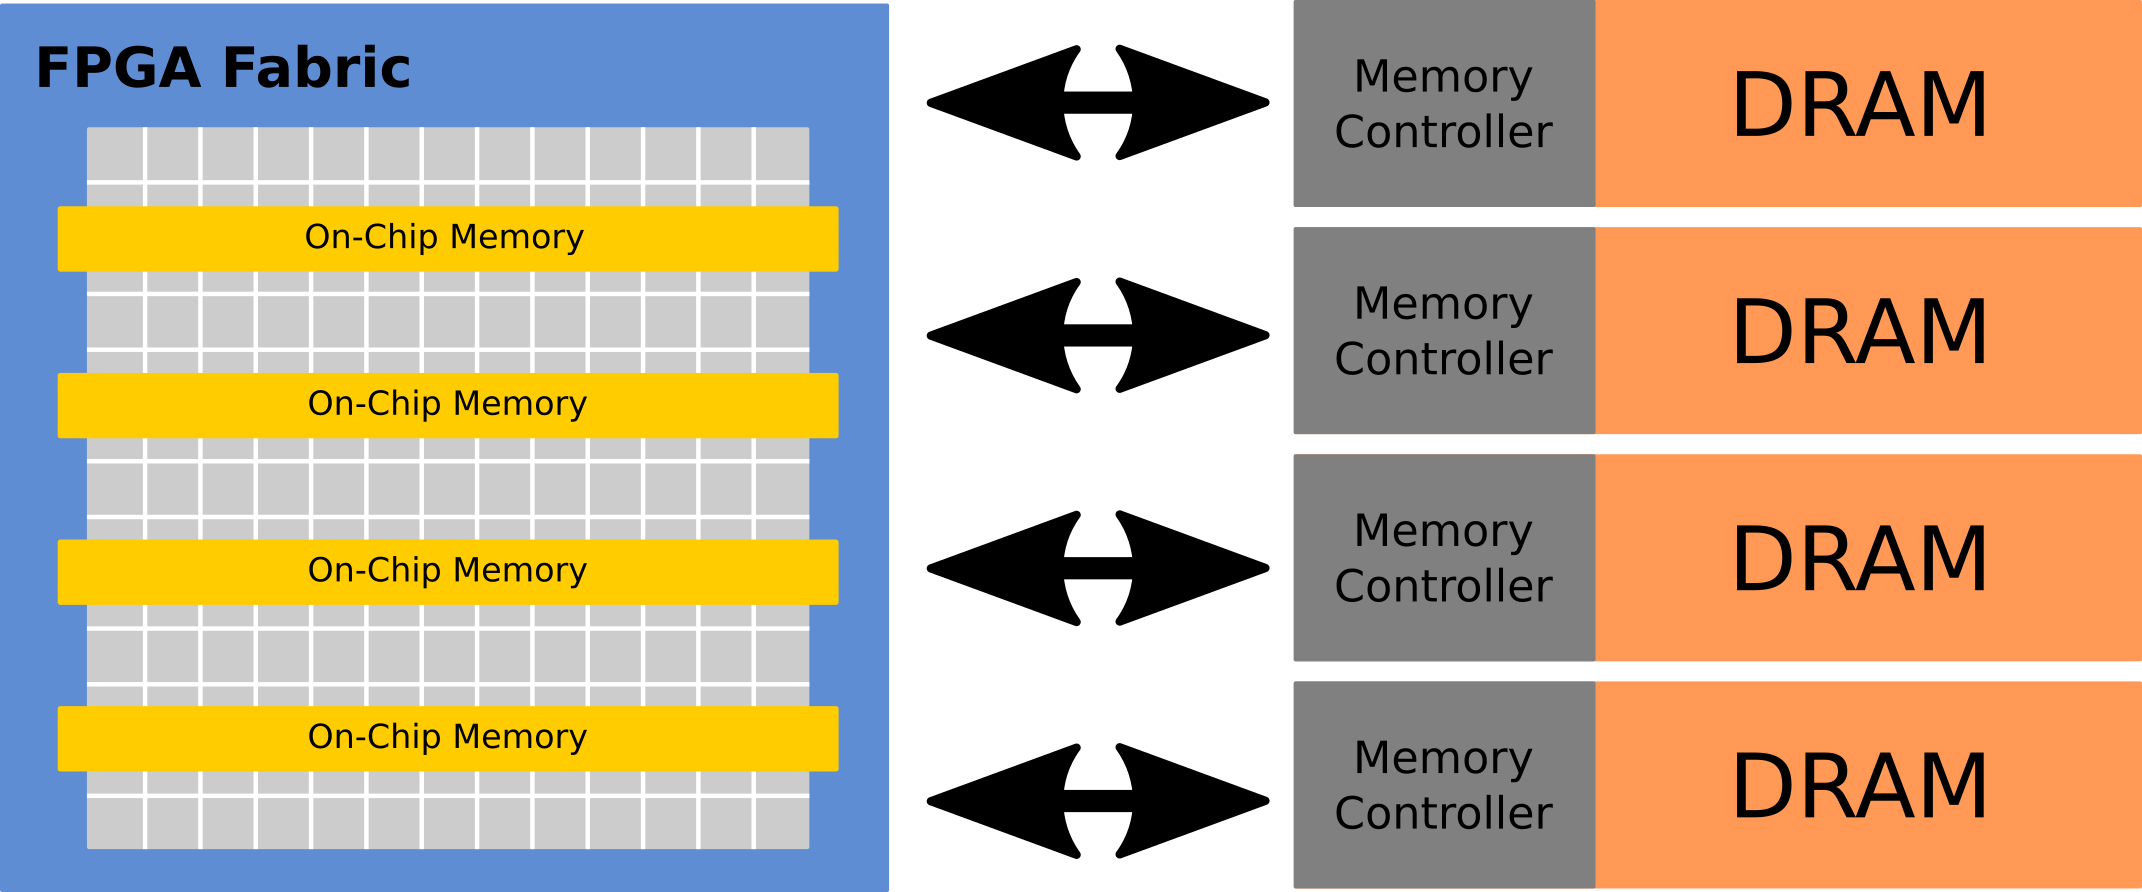
\includegraphics[height=12em]{drawings/optimizer-memory-system.png}
	\caption{High level overview of the abstracted FPGA with the key resources: fast/slow memory and memory bandwidth.}
	\label{fig:optimizer-memory-system2}
\end{figure}

\section{Approach}
We start our algorithm by putting all buffers (internal and delay) into fast memory. Then, we swap out the buffer that uses the memory \textit{most inefficiently} to slow memory. We repeat this till we reach the goal of the strategy chosen. We will walk through an example to get an intuition of the decision for the right choice of swapping out.


\paragraph{Most Inefficient Buffer}
We move the buffer with the highest metric \\ $\frac{\textrm{memory size(buffer)}}{\textrm{communication volume(buffer)}}$) from fast to slow memory. In other words, we "pay" communication volume and slow memory (we do not bother about the slow memory, since this is usually orders of magnitudes larger than the fast memory) for getting rid of some amount of buffer space. The buffer with the highest metric value get is optimal to swap out, since we "pay" the least amount compared to the size of the buffer we can remove from fast memory. \\
Since the communication volume of a buffer depends on the predecessor and successors location in memory, we will walk through an example to derive the rule for calculating the actual value. 


\subparagraph{Initial state}
In figure \ref{fig:optimizer-all-fast-memory} you can see the channel from the input kernel to the next kernel, split up into the delay buffer and the junks of the internal buffer (each part is from one field access to the next). For example a kernel \textit{out[i] = in[i-2] + in[i] + in[i+10]} would have one delay buffer and the internal buffer split into two parts of size 2 and 10. At the moment, they are all allocated in fast memory. We will analyze the communication volume for the darker part of the internal buffer dependent on the location of its predecessor and successor. \\
We can observe that the communication volume imposed by our buffer is zero if the predecessor and successor are in located in fast memory too. 



\subparagraph{Swap Out of Marked Buffer}
We moved out the marked buffer to slow memory (figure \ref{fig:optimizer-main-slow-memory}), which imposes an additional communication volume of $2*X*Y*Z$ 

\begin{figure}[h]
	\begin{minipage}{.5\columnwidth}
		\centering
		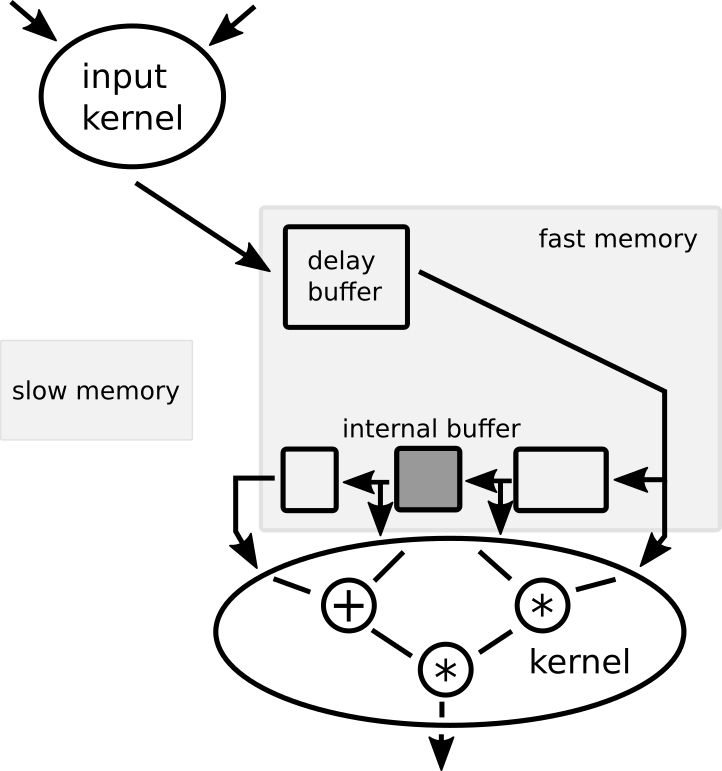
\includegraphics[height=16em]{drawings/optimizer-all-fast-memory.png}
		\caption{Scenario 1: All buffers are allocated in fast memory.}
		\label{fig:optimizer-all-fast-memory}
	\end{minipage}
	\begin{minipage}{.5\columnwidth}
		\centering
		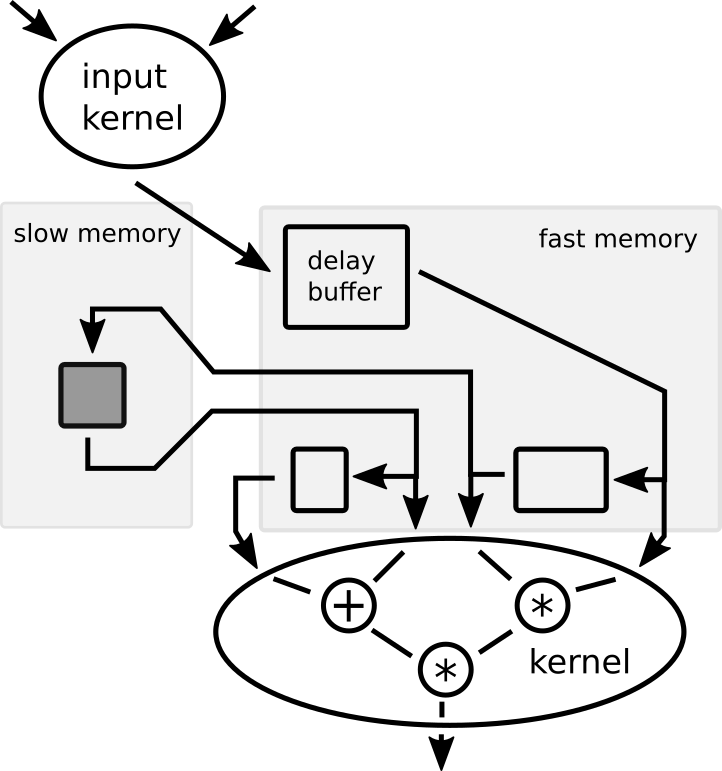
\includegraphics[height=16em]{drawings/optimizer-main-slow-memory.png}
		\caption{Scenario 2: The marked internal buffer is in slow memory but its predecessor and successor are in fast memory.}
		\label{fig:optimizer-main-slow-memory}
	\end{minipage}
\end{figure}

\subparagraph{Swap Out Successor}
This time, the successor of the marked buffer was already allocated in slow memory while the predecessor is still allocated in fast memory as shown in figure \ref{fig:optimizer-main-succ-slow-memory}. Moving out the marked buffer to slow memory imposes an additional communication volume of $1*X*Y*Z$. 


\subparagraph{Swap Out Predecessor and Successor}
Figure \ref{fig:optimizer-prev-main-succ-slow-memory} shows a situation where the predecessor and the successor have both already been swapped out. Swapping out the marked buffer in this situation actually does not impose any additional communication volume. The only thing changing is the direction of data movement (The output of the marked buffer was going from fast to slow, and now it goes into opposite direction)  
\begin{figure}[h]
	\begin{minipage}{.5\columnwidth}
		\centering
		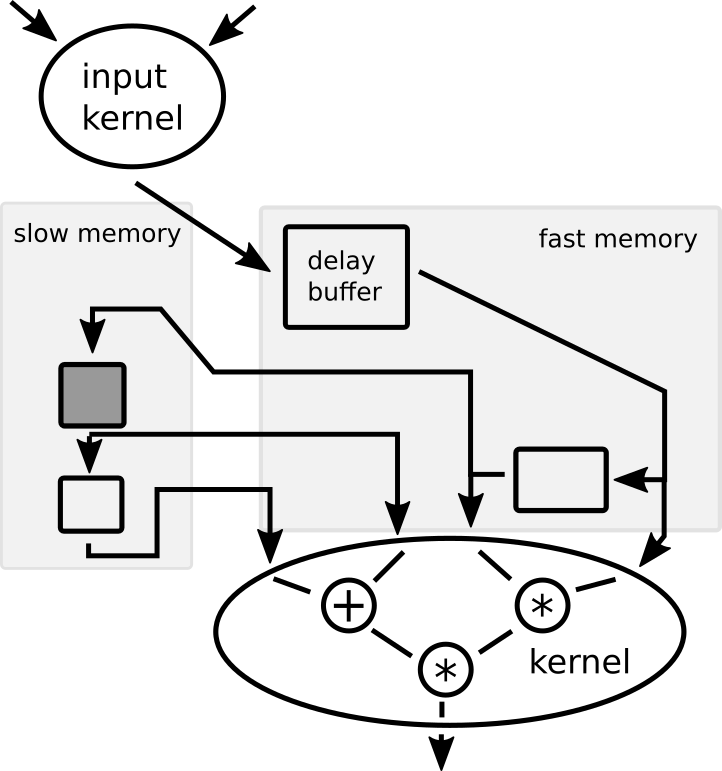
\includegraphics[height=16em]{drawings/optimizer-main-succ-slow-memory.png}
		\caption{Scenario 3: The marked internal buffer is in slow memory with its successor. The predecessor is allocated in fast memory.}
		\label{fig:optimizer-main-succ-slow-memory}
	\end{minipage}
	\begin{minipage}{.5\columnwidth}
		\centering
		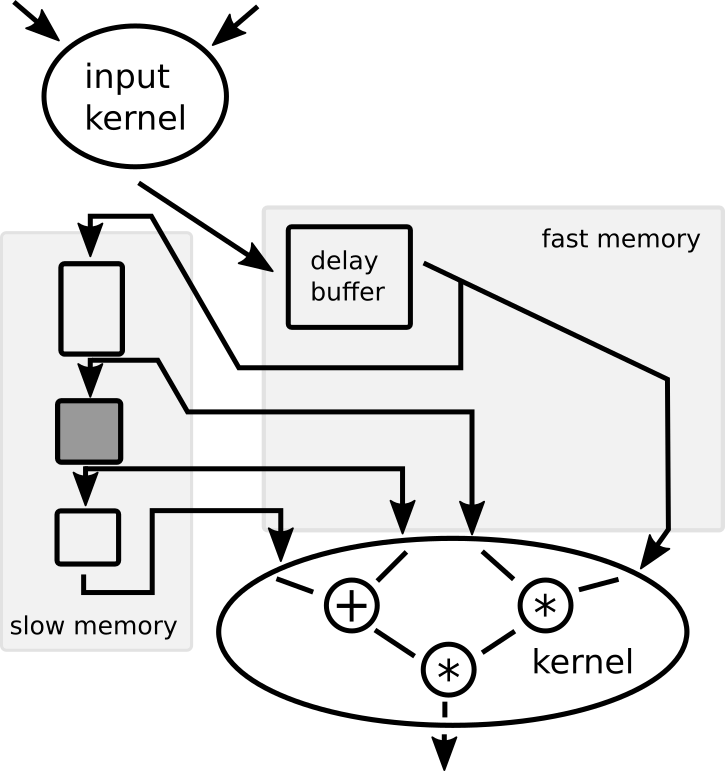
\includegraphics[height=16em]{drawings/optimizer-prev-main-succ-slow-memory.png}
		\caption{Scenario 4: The marked internal buffer is in slow memory together with its predecessor and successor.}
		\label{fig:optimizer-prev-main-succ-slow-memory}
	\end{minipage}
\end{figure}


\subparagraph{Conclusion}
The general rule for swapping the buffer out as explained in the previous example is given by: 
pre=predecessor
suc=successor
global array size = X*Y*Z = C
\begin{itemize}
	\item pred and succ in fast mem: 2*C
	\item pred in fast, succ in slow mem: C
	\item pred in slow, succ in fast mem: C
	\item pred and succ in slow mem: 0
\end{itemize}

\subparagraph{Optimizer}
On a high level, the optimizer works as follow:
\begin{algorithm}
	\caption{Optimizer}
	\begin{algorithmic}
		\WHILE{objective\_not\_reached}
		\STATE find buffer with highest metric value
		\STATE swap the buffer out
		\STATE update communication volume metric values for 
		\STATE its neighbors 
		\ENDWHILE
	\end{algorithmic}
\end{algorithm}


\section{Strategies}
Even though we have a fixed objective and a clear understanding on how we optimize, there are several scenarios with different requirements we can optimize for. 


\subparagraph{Minimization of Communication Volume}
Reduction of communication volume implies maximal usage of the fast on-chip memory resources and reduces data movement which is a natural choice of optimization.


\subparagraph{Minimization of Fast Memory}
Minimization of fast memory is a favorable strategy for example if one wants to use the remaining fast memory for other purposes. One such scenario would be tiling. 


\subparagraph{Optimization to Ratio}
This optimization strategy tries to optimize the buffer allocations in the best way to fit the ratio $\frac{\textrm{fast memory}}{\textrm{communication volume}}$ while staying below the upper bound of communication volume. This is a very useful metric if we assume that the DRAM (slow memory) is not our limiting factor and want to find out how many devices are required to fit the whole design onto it. If we choose the ratio of $\frac{\textrm{fast memory}}{\textrm{communication volume}}$ for a particular hardware device, we can reason about the number of devices required to implement our design as: $\textrm{number of required devices} = \frac{\textrm{fast memory size after optimization}}{\textrm{fast memory on a single device}}$
